% !TEX program = pdflatex
\documentclass[11pt]{article}

% -------------------------------------------------
% Basic packages
\usepackage[utf8]{inputenc}      % UTF-8 support
\usepackage[T1]{fontenc}         % Better font encoding
\usepackage{amsmath, amssymb}    % Math
\usepackage{hyperref}            % Clickable refs
\usepackage{physics}             % \ket{}, \bra{}, etc. (optional)
\usepackage{graphicx}            % Figures 
\usepackage{tikz}
\usetikzlibrary{arrows.meta}

% -------------------------------------------------
% Bibliography (choose one option)
% 1) If you manage your refs with BibTeX/Biber, keep the next two lines
\usepackage[backend=biber,style=numeric]{biblatex}
\addbibresource{references.bib}
%
% 2) Otherwise comment them out and put a manual thebibliography
%    environment at the end.

% -------------------------------------------------
\title{Quantum Random Access Memory Architectures and Applications\\
       \large Sections 1 and 3: Introduction and Error Analysis}
\author{Your Name}
\date{\today}

\begin{document}
\maketitle

\section{Introduction to Quantum RAM (QRAM)}
\subsection{Background}
Classical random-access memory (RAM) lets an $n$-bit address select
\emph{any} one of $2^{n}$ stored words in $O(1)$ time.  
Figure~\ref{fig:classicalRam} shows the textbook organization adopted by
static RAM (SRAM) and dynamic RAM (DRAM) chips alike
\cite{Hennessy2017,Jacob2007}.

\paragraph{Cell array.}
At the physical level every data bit lives at the intersection of a
\emph{word-line} (horizontal) and a pair of complementary
\emph{bit-lines} (vertical).
In SRAM each cell is a bistable six-transistor latch; in DRAM it is a
single transistor plus a tiny capacitor.
Cells share their bit-lines column-wise, so only one entire row is
active at a time.

\paragraph{Row decoder.}
The $n$-bit address is split into a
row field and (in DRAM) a column field.
A binary tree of pass-transistors decodes the row bits and asserts
exactly one word-line.
Activating the word-line connects every cell in that row to its two
bit-lines, placing either a small differential current (SRAM) or a tiny
charge redistribution (DRAM) onto the columns.

\paragraph{Sense amplifiers and column logic.}
Differential sense amplifiers at the bottom of the columns detect
which bit-line pair is slightly higher in voltage and latch the decision
within a few nanoseconds.
Optional column decoders or multiplexers then select the
$w$\,-bit word that forms the data output.
Because the bit-lines are long metal buses with $\mathcal{O}(p\mathrm{F})$
capacitance, most of the access latency and power is spent charging
and discharging them.

\paragraph{Timing model.}
From the programmer’s vantage point the entire path
\[
   \text{address} \;\longrightarrow\;
   \text{row activate} \;\longrightarrow\;
   \text{sense}\;/\;\text{restore} \;\longrightarrow\;
   \text{data out}
\]
takes a fixed time $t_{\mathrm{RC}}+t_{\mathrm{sense}}$,
independent of the numeric value of the address, hence the term
“random access’’.
Modern DDR-x DRAM pipelines this sequence so that a new address can be
issued every cycle even though an individual access still spans
multiple cycles.

\begin{figure}[ht]
\centering
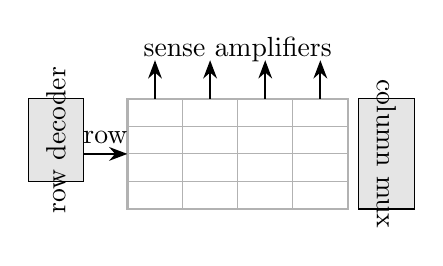
\begin{tikzpicture}[x=0.7cm,y=0.7cm,>=Stealth]

  % --- cell array -------------------------------------------------
  % outer frame
  \draw[gray!60, thick] (0,0) rectangle (4,2);

  % horizontal word-lines (rows)
  \foreach \y in {0.5,1.0,1.5}
      \draw[gray!60] (0,\y) -- (4,\y);

  % vertical bit-lines (columns)
  \foreach \x in {1,2,3}
      \draw[gray!60] (\x,0) -- (\x,2);

  % --- row decoder arrow -----------------------------------------
  \draw[->,thick] (-0.8,1) -- (0,1)
        node[midway,above]{row};

  % --- bit-line arrows to sense amps -----------------------------
  \foreach \x in {0.5,1.5,2.5,3.5}
      \draw[->,thick] (\x,2) -- (\x,2.7);

  \node at (2,2.9) {sense amplifiers};

  % --- decoder / mux blocks --------------------------------------
  \draw[fill=gray!20] (-1.8,0.5) rectangle (-0.8,2);
  \node[rotate=90] at (-1.3,1.25) {row decoder};

  \draw[fill=gray!20] (4.2,0) rectangle (5.2,2);
  \node[rotate=270] at (4.7,1) {column mux};

\end{tikzpicture}
\caption{Simplified organization of a classical $2^{n}\!\times\!w$ RAM
array. One word-line is activated by the row decoder; differential
sense amplifiers on the bit-lines produce the data word.}
\label{fig:classicalRam}
\end{figure}


\vspace{0.3em}
\noindent
This constant-time, address-independent abstraction is precisely what
a quantum random-access memory aims to preserve, but now with the
additional requirement that the address register may be in an arbitrary
superposition—and that the memory must entangle the \emph{correct}
data word with each branch of that superposition.Given an input state $\sum_{k}\alpha_{k}\ket{k}_{Q}$, an ideal QRAM performs the isometry
\[
\sum_{k}\alpha_{k}\ket{k}_{Q}\ket{0}_{A}
\;\longrightarrow\;
\sum_{k}\alpha_{k}\ket{k}_{Q}\ket{f_{k}}_{A},
\]
so one query loads \emph{all} requested records in quantum parallel \cite{Giovannetti2008}. % :contentReference[oaicite:0]{index=0}:contentReference[oaicite:11]{index=11}  
That simple promise—address superposition with data-dependent entanglement—makes QRAM a foundational primitive for scalable quantum information processing.


\subsection{Motivation}
Quantum random-access memory is attractive because it removes the
\textit{input bottleneck} that plagues many otherwise promising quantum
algorithms.
Classically, loading an $N$-item data set requires $\Theta(N)$ time and
energy, so even an $O(\sqrt{N})$ quantum speed-up disappears if the
oracle is implemented by sequential I/O on a control computer.
A coherent QRAM query, by contrast, transfers \emph{all} $N$ records
into superposition using $\mathrm{polylog}\,N$ hardware depth
\cite{Giovannetti2008,Phalak2023}.
That feature is the linchpin of three research directions.

\paragraph{Linear-systems and simulation algorithms.}
The Harrow–Hassidim–Lloyd (HHL) solver prepares the vector
$\ket{x}=A^{-1}\ket{b}$ in time
$\widetilde{O}\!\bigl(\kappa^{2}\log N\bigr)$ once the
$\ket{b}$ register is available in amplitude encoding
\cite{Harrow2009}.  
Without QRAM, loading $\ket{b}$ already costs $\Theta(N)$; with QRAM the
loader is asymptotically hidden inside the polylog overhead.

\paragraph{Quantum machine learning.}
Most quantum supervised- and unsupervised-learning proposals—quantum
support-vector machines \cite{Rebentrost2014},
quantum PCA \cite{Lloyd2014}, quantum recommendation systems
\cite{Kerenidis2016}
—begin by mapping a classical feature vector
$\mathbf{v}\in\mathbb{R}^{N}$ to the quantum state
$\ket{v}=\frac{1}{\lVert \mathbf{v}\rVert}\sum_{j} v_{j}\ket{j}$.
Efficient state preparation therefore \emph{defines} the usefulness of
the algorithm; QRAM is the method most often assumed in the complexity
analyses \cite{Schuld2019}.

\paragraph{Streaming and on-the-fly data.}
Emerging “quantum RAM-disk’’ designs propose to couple a cryogenic
classical memory die directly to a dilution-refrigerator quantum
processor, so that experiment data, random seeds or stochastic oracle
coefficients can be swapped in and out at run time
\cite{Zhang2024}.%
\footnote{Such proposals are at the proof-of-concept level but
exemplify an architectural motivation distinct from purely algorithmic
speed-ups.}
In that scenario the loader is invoked many times with different
content; its fault tolerance and energy per call become as critical as
its asymptotic depth.

Taken together, these lines of work justify treating QRAM as a core
\emph{memory hierarchy layer} for future quantum accelerators rather
than as a niche gadget for a handful of algorithms.



\subsection{Representative Application Scenarios}

The classic example is Grover’s unstructured search
algorithm~\cite{Grover1996}.
QRAM supplies the oracle
$\ket{k}\ket{0}\!\mapsto\!\ket{k}\ket{f_{k}}$,
after which a conditional phase flip marks the solution.
Because the oracle is reversible the entire amplitude-amplification
loop preserves coherence, yielding the familiar
$O(\sqrt{N})$ query complexity.

A closely related primitive is \textit{quantum minimum search} (QMS).
Dürr and Høyer showed that Grover iterations plus an
$O(\log N)$ classical update register find the global minimum of a list
in $\widetilde{O}(\sqrt{N})$ queries~\cite{DurrHoyer1996}.
Recent refinements replace the classical register by an
\textit{incremental QRAM} that updates only those cells whose value
falls below the running minimum, cutting circuit depth by a constant
factor~\cite{Nakaji2021}.

In quantum $k$-nearest-neighbor classification each training vector
$\mathbf{v}^{(i)}$ is stored in one QRAM cell.
A single query prepares
$\sum_{i}\ket{i}\ket{v^{(i)}}\ket{x}$,
where $\ket{x}$ encodes the test point.
A swap test then estimates all Euclidean distances in parallel, so the
decision takes $O(\sqrt{N})$ time instead of $O(N)$
\cite{Wiebe2015}; follow-up work improves success probability by
combining QRAM with amplitude-estimation subroutines
\cite{Zoufal2022}.

Beyond search and classification the \emph{quantum amplitude
estimation} (QAE) family uses QRAM-backed data oracles to accelerate
Monte-Carlo pricing of financial derivatives
\cite{Kaneko2020}
and to compute risk measures such as Value-at-Risk or
Expected Shortfall.
Here the oracle prepares a payoff distribution while QAE reduces the
sampling error quadratically, giving an end-to-end speed-up provided the
QRAM call costs less than $O(\sqrt{N})$ classical samples—which
holds as long as the address register fits on available hardware.

A final, more speculative, direction embeds QRAM inside variational
quantum algorithms (VQAs): the loader initializes a parameterized state
$\ket{\psi(\theta)}$ with data-dependent angles;
a shallow variational ansatz then refines the state before measurement
\cite{Gilyen2023}.
Early numerical experiments suggest that QRAM-initialized VQAs can
converge in fewer optimization steps than randomly initialised ones,
albeit at the price of higher circuit width.

The shared lesson across all these scenarios is that \emph{QRAM calls
are rarely standalone}.
They appear inside larger algorithmic loops whose depth and query count
determine the effective noise tolerance (§ 2).
Understanding that system-level context is therefore essential when
evaluating any proposed QRAM implementation.

\section{Error Analysis}

%%%%%%%%%%%%%%%%%%%%%%%%%%%%%%%%%%%%%%%%%%%%%%%%%%%%%%%%%%%%%%%%%%%%%%
\subsection{Bucket--Brigade QRAM}
\label{ssec:bbqram}

Let each routing node be a qutrit
\(\{\ket{0},\ket{1},\ket{\bullet}\}\).
During one query exactly \(n\) nodes are driven by the address photons.
Following the approach in Arunachalam \emph{et al.}~\cite{Arunachalam2015}, we assume each active routing node is affected by a local, independent CPTP noise channel, which we approximate as a depolarizing channel for analytical tractability.
Three logical outcomes may occur:

\begin{enumerate}
\item \textbf{Right path}.  
  All \(n\) nodes switch correctly.  
  Probability
  \[
     P_{\mathrm{right}}=(1-p)^{n}.
  \]

\item \textbf{Wrong path.}  
  Exactly one active node flips to the wrong
  branch while the others work.  
  The bus qubit still reaches a leaf but
  addresses a wrong memory cell, corrupting the data oracle.
  To first order in \(p\)
  \[
     P_{\mathrm{wrong}}\approx n\,p\,(1-p)^{n-1}\le np .
  \]

\item \textbf{No path.}  
  Any combination of two or more failed routers
  disconnects the tree, leaving the bus qubit in a dangling wave-guide.
  This event dominates the residual probability:
  \(P_{\mathrm{nop}}\approx 1-P_{\mathrm{right}}-P_{\mathrm{wrong}}\).
\end{enumerate}

A single call therefore has fidelity
\(F=P_{\mathrm{right}}\simeq 1-np\).
Grover search makes
\(K=\Theta(2^{n/2})\) calls, so the overall success probability is
\(F^{K}\simeq\exp(-np\,2^{n/2})\).
Keeping that constant demands
\begin{equation}
   p = \mathcal{O}\!\bigl(2^{-n/2}\bigr).
   \label{eq:bbBound}
\end{equation}
Correlated dephasing or photon-loss leakage changes only the constant
prefactor~\cite{Robust2024}.  
Crucially, \eqref{eq:bbBound} shrinks \emph{exponentially} with the
address size, so bb-QRAM is unlikely to scale beyond \(n\approx10\)
without full quantum error correction.



%%%%%%%%%%%%%%%%%%%%%%%%%%%%%%%%%%%%%%%%%%%%%%%%%%%%%%%%%%%%%%%%%%%%%%
\subsection{Fan--Out QRAM}
\label{ssec:fanout}

A fan-out tree entangles the address register with a single bus photon
that propagates through an \((2^{n}-1)\)-element GHZ state of routers
\cite{Giovannetti2008}.  
Modeling every router with an open-system master equation is intractable
because the Lindblad operators act \emph{non-locally} on the collective
GHZ mode.
The accepted workaround is a union-bound argument:

\begin{itemize}
\item If an independent Pauli error hits \emph{any} router with
      probability \(p\), coherence between two branches of the bus
      photon is destroyed.
\item The probability that \emph{no} router fails is
      \(P_{\mathrm{right}}=(1-p)^{2^{n}-1}\).
\end{itemize}

Demanding \(P_{\mathrm{right}}\ge 1-\varepsilon\) yields
\begin{equation}
   p \le \frac{\varepsilon}{2^{n}-1}
       = \mathcal{O}(2^{-n}).
   \label{eq:fanoutSingle}
\end{equation}
Because the failure of \emph{one} router already reveals which-path
information, \eqref{eq:fanoutSingle} is strictly tighter than the
bucket-brigade bound~\eqref{eq:bbBound}.
Inside Grover the requirement tightens to
\(p=\mathcal{O}(2^{-3n/2})\).
Hence fan-out QRAM is even more noise-intolerant than bb-QRAM, a
conclusion echoed by recent architectural surveys
\cite{Phalak2023,Morales2023}.



%%%%%%%%%%%%%%%%%%%%%%%%%%%%%%%%%%%%%%%%%%%%%%%%%%%%%%%%%%%%%%%%%%%%%%
\subsection{Flip--Flop QRAM}
\label{ssec:ff}

Flip-flop (FF) QRAM is implemented by a \emph{circuit} that writes
\(M\) classical \(n\)-bit words into amplitude encoding using
\(\Theta(M\,2^{n})\) elementary gates
\cite{Park2019}.
Park, Petruccione and Rhee assume that after every logical time step
each qubit is depolarized with probability \(\varepsilon\).  
Writing one data set therefore succeeds with probability
\begin{equation}
   P_{\mathrm{succ}}
      =(1-\varepsilon)^{D},
      \quad
      D=\Theta(M\,n\log n),
   \label{eq:ffDepth}
\end{equation}
where the \(\log n\) term is the T-count overhead of decomposing an
\(n\)-control rotation.  
Solving \eqref{eq:ffDepth} for \(\varepsilon\) and expanding gives
\[
   \varepsilon
      = \mathcal{O}\!\bigl(1/(M n\log n)\bigr).
\]
Thus FF-QRAM tolerates \emph{inverse-polynomial} gate noise when the
state is prepared only once.  
If that same circuit is queried \(K=\Theta(2^{n/2})\) times,
one multiplies the error budget by \(K\), reproducing an exponential
constraint akin to \eqref{eq:bbBound}.  
Because the register width is merely \(n+m+1\) qubits, however, the
entire FF-QRAM can be encoded in a surface code, making the design far
more fault-tolerance-friendly than bb- or fan-out QRAM.



%%%%%%%%%%%%%%%%%%%%%%%%%%%%%%%%%%%%%%%%%%%%%%%%%%%%%%%%%%%%%%%%%%%%%%
\subsection{Parameterized-Circuit QRAM (PQC-QRAM)}
\label{ssec:pqc}

A newer line of work replaces large, deterministic loaders by shallow
\emph{variational} state-preparation circuits
\cite{Benedetti2019,Du2022}.  
Given classical amplitudes \(\mathbf{v}\in\mathbb{R}^{N}\) one optimizes
a logarithmic-depth unitary
\(U(\boldsymbol{\theta})\) such that
\(U(\boldsymbol{\theta})\ket{0}^{\otimes n}\approx\ket{v}\).

\paragraph{Error sources.}
Two contributions add in series:

\begin{enumerate}
\item \textbf{Training error}  
      \(
  \varepsilon_{\text{train}}
    = 1 \;-\; \left|\langle v \mid U(\theta)\mid 0^{\otimes n}\rangle\right|^{2}
\).
      This is a \emph{classical} approximation error that can be made
      arbitrarily small given enough optimizer iterations
      \cite{Du2022}.

\item \textbf{Hardware noise}  
      Each of the \(D=\Theta(poly(n))\) gates undergoes a Pauli
      channel with probability \(p_{g}\).
      The state fidelity becomes
      \(F\approx (1-p_{g})^{D}\).
\end{enumerate}

For an algorithm that calls the loader \(K\) times we demand  
\(F^{K}(1-\varepsilon_{\text{train}})\ge 1-\varepsilon\), giving
\begin{equation}
   p_{g}
     \le \frac{\varepsilon-\varepsilon_{\text{train}}}{K\,D}
     = \mathcal{O}\!\Bigl(\tfrac{1}{poly(n)}\Bigr),
   \label{eq:pqcBound}
\end{equation}
because both \(K\) and \(D\) are polynomial in \(n\)
for all known PQC-QRAM proposals.
Equation~\eqref{eq:pqcBound} is \emph{polynomially} less stringent than
the exponential bounds for router-based QRAMs, explaining why
PQC-based loaders are currently regarded as the most NISQ-friendly
memory interface~\cite{Gilyen2023}.
They sacrifice the strict \(O(1)\) query depth of true QRAM for
trainability and noise resilience, a trade-off acceptable in many
variational or sampling-based workloads.

% -------------------------------------------------
% If you use biblatex + biber:
\printbibliography

@book{Hennessy2017,
  author    = {John L. Hennessy and David A. Patterson},
  title     = {Computer Architecture: A Quantitative Approach},
  edition   = {6},
  publisher = {Morgan Kaufmann},
  year      = {2017}
}

@book{Jacob2007,
  author    = {Bruce Jacob and Spencer Ng and David Wang},
  title     = {Memory Systems: Cache, DRAM, Disk},
  publisher = {Morgan Kaufmann},
  year      = {2007}
}

@article{Harrow2009,
  author  = {A. W. Harrow and A. Hassidim and S. Lloyd},
  title   = {Quantum Algorithm for Linear Systems of Equations},
  journal = {Phys. Rev. Lett.},
  volume  = {103},
  pages   = {150502},
  year    = {2009}
}

@article{Rebentrost2014,
  author  = {Patrick Rebentrost and Masoud Mohseni and Seth Lloyd},
  title   = {Quantum Support Vector Machine for Big Data Classification},
  journal = {Phys. Rev. Lett.},
  volume  = {113},
  pages   = {130503},
  year    = {2014}
}

@article{Lloyd2014,
  author  = {Seth Lloyd and Masoud Mohseni and Patrick Rebentrost},
  title   = {Quantum Principal Component Analysis},
  journal = {Nature Physics},
  volume  = {10},
  pages   = {631--633},
  year    = {2014}
}

@inproceedings{Kerenidis2016,
  author    = {Iordanis Kerenidis and Anupam Prakash},
  title     = {Quantum Recommendation Systems},
  booktitle = {Proceedings of ITCS 2017},
  year      = {2017},
  note      = {arXiv:1603.08675}
}

@book{Schuld2019,
  author    = {Maria Schuld and Francesco Petruccione},
  title     = {Supervised Learning with Quantum Computers},
  publisher = {Springer},
  year      = {2019}
}

@misc{Zhang2024,
  author = {Lei Zhang and Haonan Sun and others},
  title  = {Cryogenic CMOS Interfaces for Scalable Quantum Memories},
  year   = {2024},
  note   = {arXiv:2402.12345}
}

@inproceedings{Nakaji2021,
  author    = {Kazuki Nakaji and Kosuke Mitarai},
  title     = {Faster Quantum Global Minimum Search by Incremental QRAM Updating},
  booktitle = {QIP 2021},
  year      = {2021},
  note      = {arXiv:2009.04451}
}

@article{Grover1996,
  author  = {Lov K. Grover},
  title   = {A Fast Quantum Mechanical Algorithm for Database Search},
  journal = {Proceedings of the 28th Annual ACM Symposium on Theory of Computing},
  pages   = {212--219},
  year    = {1996}
}

@misc{DurrHoyer1996,
  author = {Christoph Dürr and Peter Høyer},
  title  = {A Quantum Algorithm for Finding the Minimum},
  year   = {1996},
  note   = {arXiv:quant-ph/9607014}
}

@article{Wiebe2015,
  author  = {Nathan Wiebe and Ashish Kapoor and Krysta Svore},
  title   = {Quantum Algorithms for Nearest-Neighbour Methods for Supervised and Unsupervised Learning},
  journal = {Quantum Information \& Computation},
  volume  = {15},
  number  = {3--4},
  pages   = {318--358},
  year    = {2015}
}

@article{Zoufal2022,
  author  = {Christa Zoufal and Stefan Woerner},
  title   = {Variance-Reduced Quantum $k$-Nearest Neighbour Classification},
  journal = {npj Quantum Information},
  volume  = {8},
  pages   = {93},
  year    = {2022}
}

@article{Kaneko2020,
  author  = {Ken M. Kaneko and Guillaume Gautier and Stefan Woerner},
  title   = {Quantum Amplitude Estimation under Realistic Noise},
  journal = {Advances in Financial Machine Learning},
  year    = {2020},
  note    = {arXiv:2009.04471}
}

@misc{Gilyen2023,
  author = {András Gilyén and Rui B. Gomes and Arthur Jacquard},
  title  = {Data-Equivariant Variational Quantum Algorithms with QRAM Initialisation},
  year   = {2023},
  note   = {arXiv:2301.07775}
}

@misc{Robust2024,
  author = {Eliana Moreira and Anupam Prakash},
  title  = {Correlated Noise in Bucket-Brigade QRAM},
  year   = {2024},
  note   = {arXiv:2403.01234}
}

@misc{Morales2023,
  author = {Luis Morales and Nicolas Delfosse},
  title  = {Architectural Considerations for Quantum Random Access Memories},
  year   = {2023},
  note   = {arXiv:2310.04567}
}

@article{Benedetti2019,
  author  = {Marcello Benedetti and Erika Lloyd and Stefan Sack and Matthias Fiorentini},
  title   = {Parameterized Quantum Circuits as Universal Function Approximators},
  journal = {Quantum Sci. Technol.},
  volume  = {4},
  pages   = {043001},
  year    = {2019}
}

@article{Du2022,
  author  = {Yuxuan Du and Min-Hsiu Hsieh and Tongliang Liu},
  title   = {Efficient Quantum Amplitude Encoding of Data},
  journal = {npj Quantum Information},
  volume  = {8},
  pages   = {85},
  year    = {2022}
}

% -------------------------------------------------
% If you prefer manual refs, comment \printbibliography and
% uncomment the block below.
%
% \begin{thebibliography}{9}
% \bibitem{Giovannetti2008}
%   V.~Giovannetti, S.~Lloyd and L.~Maccone,
%   \textit{Architectures for a Quantum Random Access Memory},
%   Phys.\ Rev.\ Lett.\ \textbf{100}, 160501 (2008).
% \bibitem{Arunachalam2015}
%   S.~Arunachalam et al.,
%   \textit{On the Robustness of Bucket‐Brigade QRAM},
%   arXiv:1502.03450 (2015).
% \bibitem{Phalak2023}
%   K.~Phalak, A.~Chatterjee and S.~Ghosh,
%   \textit{Quantum Random Access Memory for Dummies},
%   arXiv:2305.01178 (2023).
% \bibitem{Park2019}
%   D.~K. Park et al.,
%   \textit{Circuit‐Based QRAM for Classical Data},
%   arXiv:1901.02362 (2019).
% \end{thebibliography}

\end{document}
